\chapter{Empirical Study}\label{chapter:EmpiricalStudy}
To better understand the capabilities and limitations of 
MLLMs in generating accessible UI code, a comprehensive 
study guided by four research questions was conducted. 
In the following, the study setup and the quantitative and
qualitative results are presented.

\section{RQ1: Do MLLMs generate accessible code from UI screenshots?}
\subsection{Experiment Setup}
To evaluate the baseline capability of MLLMs in generating accessible
code from visual UI input, two widely-used MLLMs are 
selected for this study: GPT-4o and Gemini-2.0 Flash.
These models show strong performance in 
multimodal tasks and their support for image inputs make
them suitable candidates for this study.\newline
As described in section~\ref{chapter:Methodology}, the models are 
prompted with our dataset of UI screenshots and a corresponding 
task description. The task description includes a naive (plain)
prompt, which instructs the model to generate HTML/CSS code solely
based on the provided screenshot, without mentioning accessibility.

\newmdenv[
  backgroundcolor=lightgray,
  linecolor=black,
  linewidth=0.5pt,
%   roundcorner=20pt,
  innertopmargin=3pt,
  innerbottommargin=3pt,
  innerleftmargin=10pt,
  innerrightmargin=10pt,
  skipbelow=3pt,
  skipabove=3pt,
]{roundedbox}

\begin{roundedbox}
\textbf{Native Prompt}: Your task is to replicate 
the provided UI screenshot of a webpage pixel-perfectly using 
HTML/CSS.
\end{roundedbox}

This setups allows to observe whether MLLMs can 
naturally produce accessible code without direct instruction 
and acts as a benchmark for enhancement strategies. 
It is important to note that each experiment is conducted three 
times for each model, and the results presented represent the average 
outcomes to account for stochastic fluctuations in the model's responses.


\subsection{Results}
Both models show a strong performance in reconstructing the given 
UI layouts with an average of 88.96\% in code similarity
for GPT and 87.12\% for Gemini, as shown in table~\ref{tab:table-performance}.
These results demonstrate that the models are capable of generating 
valid and visually similar HTML/CSS code from UI screenshots. 
While a more detailed evaluation of the visual fidelity is beyond 
the scope of this thesis, these results serve as a baseline 
for subsequent accessibility analysis.
Table~\ref{tab:table-performance} presents the amount of accessibility 
violations in UI code generated by GPT and Gemini. Despite 
achieving high layout and structural fidelity, both models produce 
a significant number of accessibility issues. On average, GPT 
generates 13.75 violations per UI, while Gemini produces 12.4\% 
more. The IR is 12.22\% for GPT and 11.42\% for Gemini,
while IWIR is 47.10\% and 47.70\%, respectively. Although Gemini yields
more total violations than GPT on average, an analysis of its DOM-size 
reveals that it generates larger code snippets, which explains
its lower IR because the violations are distributed over a larger 
amount of nodes. However, the IWIR stays consistent across the two models, 
suggesting that the severity of the violations is similar.
These findings demonstrate a clear gap between visual correctness and 
accessibility compliance and highlights that without clear and 
explicit instructions, MLLMs might not be able to follow 
accessibility principles in code generation. In order to understand 
the underlying reasons for these accessibility issues, a manual 
analysis of the violations observed in the generated output
has been conducted. This process allows to identify recurring 
failure patterns and model limitations.

\begin{figure}
  \centering
  % \includegraphics[width=0.8\linewidth]{images/common.png}
  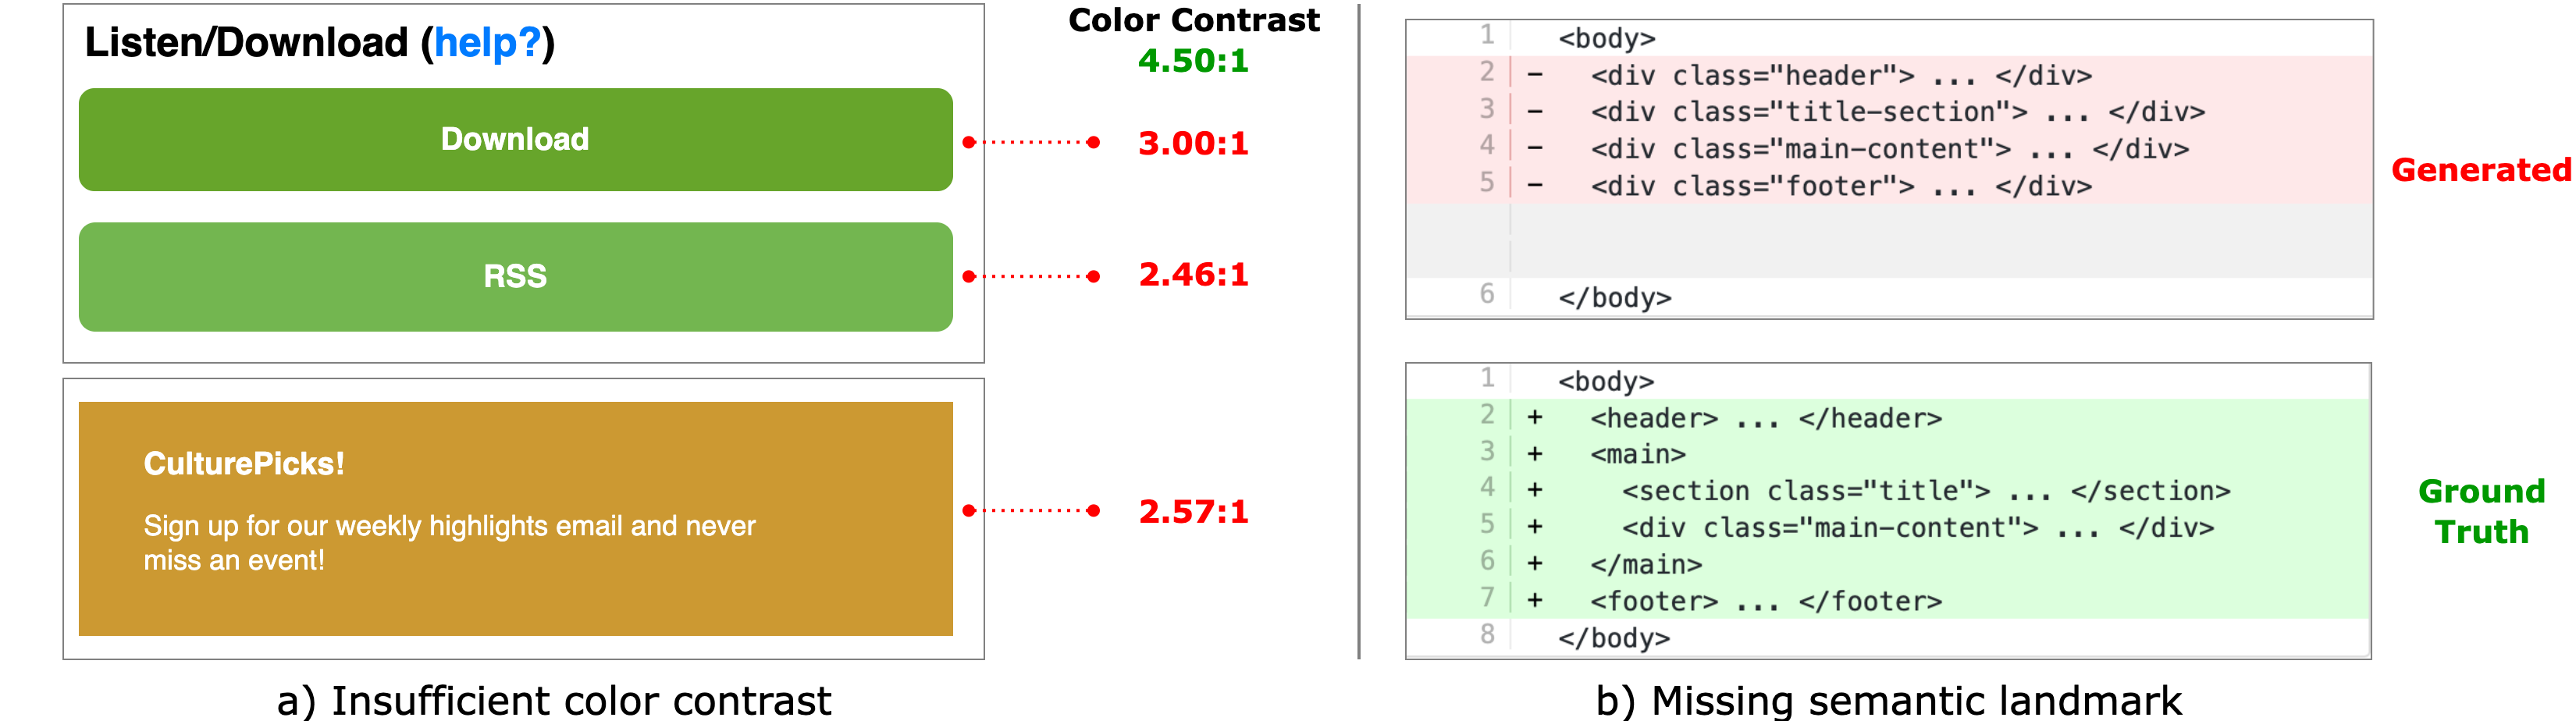
\includegraphics[width=0.9\linewidth]{figures/colorcontrastlandmarkexample.png}
  \caption{Example of common accessibility violations.}
  \label{fig:common} 
\end{figure}

\subsubsection{Most common violations}
The detailed analysis reveals that two primary categories of accessibility
issues are prevalent in the generated code across both models.
The first category is insufficient color contrast. For instance,
color contrast violations are very common, producing 5.21 violations 
per UI for GPT and 6.89 for Gemini. The reason for this frequency 
can be attributed to the complexity of contrast checking, which 
requires the model to reason mathematically about RGB or hex values
and their luminance for the human eye, defined by WCAG. This mathematical 
requirement is not only challenging for MLLMs, but also human 
developers often rely on automated tools to ensure compliance 
in this area. The main difficulty lies in the fact that 
even slight deviations in color selection can lead to significant 
usability barriers for visually impaired users. As shown in 
figure~\ref{fig:common} (a), the generated code uses a white text 
(\#ffffff) on a green background (\#67a52a and \#72b650), 
or on a yellow background (\#cc9933), which results in 
contrast ratios of 3.00, 2.46 and 2.57, significantly below the
WCAG 2.1 minimum color contrast threshold of 4.5 for normal text.
Even though this mathematical task is within the capabilities of 
MLLMs, it remains a common challenge across both models, because 
of their limited visual-perceptual understanding and mathematical 
precision.\newline
The second category is the absence or incorrect use of semantic 
landmarks. Semantic landmarks, such as \texttt{main}, \texttt{nav},
\texttt{header}, and \texttt{footer} are essential for transforming 
the visual structure of a webpage into a format used by
assistive technologies. However, these landmarks are not visually 
displayed in the UI and have no specific representation, making it 
difficult for MLLMs which rely only on screenshot input
to identify and generate them correctly. As 
shown in figure~\ref{fig:common} (b), rather than using 
semantic landmarks, the model substitutes them with 
generic \texttt{div} elements. As a result, assistive technologies 
interpret the webpage as a flat structure, lacking navigational 
and structural cues which are necessary for keyboard users or 
screen reader navigation. This can significantly hinder 
the accessibility, especially for users who rely on 
semantic segmentation to jump between regions of a page. 
Essentially, the problem arises, first, due to the absence 
of visible indicators, second, because of the model’s 
limited exposure to the underlying meaning of UI 
elements—the type of information human designers tend 
to acquire through accessibility trainings or work experience.



\begin{center}
\begin{tcolorbox}[colback=black!5!white,colframe=black!75!black,bottom=-0.05pt,top=-0.05pt]
\textit{\textbf{Finding:}} Even though both GPT and Gemini achieve high layout fidelity, 
they consistently generate code with accessibility violations, 
especially in color contrast and missing landmarks. This indicates 
a fundamental gap between visual accuracy and accessibility compliance.
\end{tcolorbox}
\end{center}


\begingroup
    \renewcommand{\arraystretch}{1.1}
\begin{table}
\tabcolsep=0.5cm
\centering
\small

\begin{tabular}{l|c|c|c|c} 
\hline
\rowcolor{lightgray} \textbf{Violations} & \textbf{GPT} & \textbf{Gemini} & \textbf{Qwen} & \textbf{Llava}  \\ 
\hline
Color contrast & 276 & 365 & 159 & 67 \\
\hline
Landmark \& Region & 279 & 265 & 114 & 187 \\
\hline
Label & 102 & 105 & 21 & 14 \\
\hline
Headings & 26 & 18 & 20 & 17 \\
\hline
Target Size & 15 & 13 & 10 & 15 \\
\hline
Distinguishable Links & 20 & 23 & 2 & 0 \\
\hline
Document Language & 0 & 11 & 0 & 0 \\
\hline
Table Headers & 1 & 7 & 1 & 0 \\
\hline
Incomplete Links & 0 & 4 & 0 & 6 \\
\hline
Image Alt-Text & 4 & 5 & 0 & 1 \\
\hline
\hline
\textbf{Total Violations} & 729 & 819 & 329 & 307 \\
\hline
\textbf{Average Violations} & 13.75 & 15.45 & 6.21 & 5.79 \\
\hline
\textbf{IR} & 12.22\% & 11.42\% & 10.70\% & 12.14\% \\
\hline
\textbf{IWIR} & 47.10\% & 47.70\% & 40.25\% & 40.40\% \\
\hline
\textbf{CodeSim} & 88.96\% & 87.12\% & 70.36\% & 50.50\% \\
\hline
\end{tabular}
\caption{Quantitative comparison of accessibility performance metrics across GPT-4o, Gemini-2.0 Flash, Qwen2.5-VL-7B, and Llava-7B.}
\label{tab:table-performance}
\end{table}
\endgroup


\section{RQ2: Do different MLLMs vary in their ability to generate accessible UI code?}
\subsection{Experiment Setup}
To understand how the choice of MLLMs influences the generation of 
accessible HTML/CSS, the analysis is extended beyond the two 
closed-sourced models used in RQ1. This included two additional 
open-source models, \textit{Qwen2.5-VL-7B} and \textit{Llava-7B}, 
selected for their strong performance in multimodal tasks and 
wide adoption in the research community. 
The 7B parameter variations are employed to capture significant 
variation in model behavior and performance while ensuring 
practicability under constrained computational resources and 
reproducibility by other researchers.
Similar to RQ1, all models are prompted with the same 
benchmark dataset and naive prompt 
which instructs the models to generate HTML/CSS from UI screenshots
without referencing accessibility. This setup allows a 
direct comparison across the models.

\subsection{Results}
Table~\ref{tab:table-performance} presents the average 
number of accessibility violations per UI, the IR, IWIR and 
CodeSim for each model. Surprisingly, the open-source models
Qwen and Llava have the fewest violations, averaging 
6.21 and 5.79 violations per UI. Also most of the other metrics 
show that these models perform better than the closed-source
models: the average values for the IR is 10.70\% for Qwen and
12.14\% for Llava, while the IWIR is 40.25\%
and 40.40\%, respectively.
Since these results 
are significantly lower than the results of GPT and Gemini, 
a closer analysis was conducted and three key factors 
influencing the accessibility results were identified: 
training data biases, instructional alignments and 
code generation capabilities.

\subsubsection{Training Data Biases.} Even if the 
internal training data of closed-source models is not publicly 
available, this qualitative analysis reveals noticeable differences 
in the models' behavior that can be attributed to the training 
data biases.\newline
The first visible difference is the tendency of Gemini to produce 
more violations related to color contrast, averaging 
6.89 per UI for Gemini, compared to 5.21, 3.00, 1.26 for GPT,
Qwen and Llava. This discrepancy seems to be closely related to 
the diversity and origin of the colors used in the generated code.
For instance, Gemini shows a relatively limited color palette, 
consisting of only 41 unique colors across all UIs that cause 
violations. Over 40\% of these violations stem from the use 
of the \textit{primary blue} (\#007bff) color, which is 
commonly used in the Bootstrap framework~\ref{web:bootstrapv4}.
This strong dependency and bias towards a specific color, suggests 
that Gemini's training data might have been disproportionately 
influenced by framework-centric codebases, such as those built 
with Bootstrap. As a result, the model shows a tendency to have 
stylistic preferences which do not align with accessibility.
For instance, the Bootstrap primary blue is often used for 
elements like links, buttons or headings, without taking the 
background color into account. Especially combined with 
light-colored layouts, this increases the risk of insufficient 
color contrast. In contrast, GPT's color contrast violations are 
caused by a set of 83 distinct colors. The majority of these 
colors (71.47\%) are uniquely synthesized by the model and can not 
be linked to any framework or library. Even if this 
independent color selection does not prevent color contrast 
violations, they tend to more closely match the visual 
design of the input UI. This can lead to improved contrast ratios,
given that the input UI is designed with accessibility in mind.
While this interpretation is speculative because of the 
black-box nature of the models, the observed patterns suggest 
a strong influence of the training data on the models' accessibility
outcomes.

\subsubsection{Instructional Alignments.} The second key 
factor appears to be the instructional alignment
and the behavior tuning of the models during training. GPT 
frequently generates code with accessibility-conscious elements
(e.g. alt-text for images or proper form labels), even when 
prompted without explicit instructions. As shown in 
figure~\ref{fig:generalcapabilities} (a), GPT tends to produce 
descriptive alt-text and labels by default.\newline
While the reasons remain speculative, a plausible explanation 
could lie in the accessibility-oriented use cases and 
alignment practices by GPT. For example, GPT has been used 
in real-world assistive technologies like \textit{Be My Eyes}. 
This application helps to interpret visual information into 
textual descriptions, which is crucial for visually impaired users.
This practical integration into a real-world scenario might 
have influenced the model's fine tuning or evaluation objectives.
These improved accessibility considerations and sensitivity could 
be a result of accessibility-focused tasks during the training 
process of the model. This characteristic is less noticeable in 
other MLLMs.

\begin{figure}
  \centering
  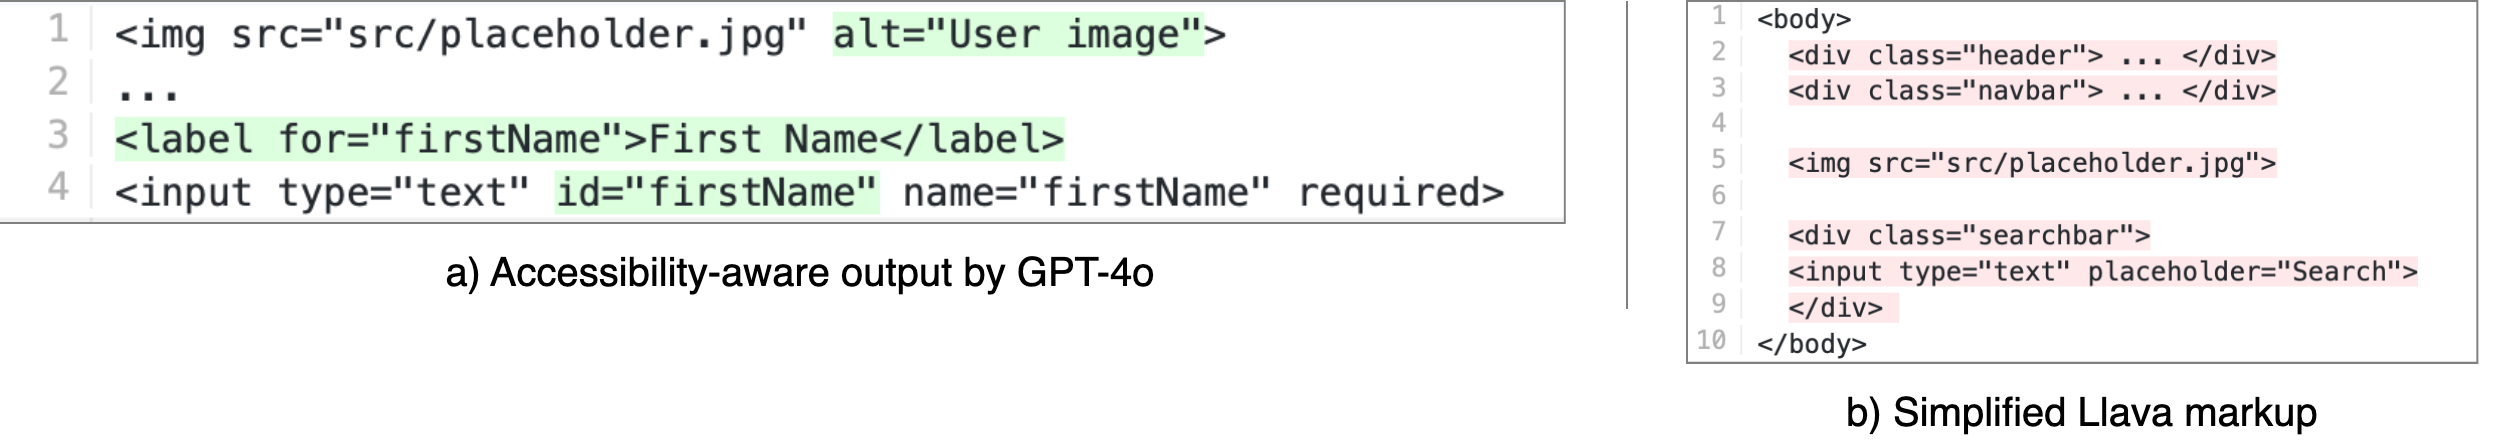
\includegraphics[width=1\linewidth]{figures/generalcapability.png}
  \caption{Comparison of semantically rich (left) and structurally shallow (right) HTML snippets}
  \label{fig:generalcapabilities} 
\end{figure}

\subsubsection{Code Generation Capabilities.} Despite generating
code with fewer violations, the open-source models Qwen and 
Llava do not necessarily produce accessible webpages.
The detailed analysis reveals that these models tend to generate 
simplistic and semantically shallow code snippets. They often 
generate flat layouts or generic tags, such as \texttt{div} or \texttt{span},
combined with little nesting, styling or ARIA annotations as default. 
This behavior is illustrated in figure~\ref{fig:generalcapabilities} (b),
where Llava reduces a multi-component UI layout into a linear 
sequence of \texttt{div} elements, following a common template.
This approach leads to fewer accessibility violations, 
because it lacks problematic elements and therefore reduces the 
surface for potential issues. However, this results in 
structurally incomplete and visually incorrect code, which can be 
seen in significant lower code similarity scores of 70.36\% for Qwen and
50.50\% for Llava, compared to 88.96\% for GPT and 87.12\% for Gemini.
This indicates that the smaller, open-source models fail to capture 
layout fidelity and semantic depth. This finding highlights the 
necessity to balance accessibility evaluation with structural 
quality, because the absence of content can artificially 
reduce the violation metrics.

\begin{center}
\begin{tcolorbox}[colback=black!5!white,colframe=black!75!black,bottom=-0.05pt,top=-0.05pt]
\textit{Finding:} Due to variations in alignment goals (e.g., GPT's accessibility-aware behavior) and training data composition (e.g., Gemini's dependence on framework-derived styles), accessibility violations differ significantly amongst MLLMs. Open-source models, such as Qwen and Llava, tend to produce simplified, under-specified code, which is the main reason why they report fewer violations.
\end{tcolorbox}
\end{center}


\section{RQ3: Does advanced prompt engineering lead to more accessible MLLM-generated
UI code?}
\subsection{Experiment Setup}
While the prior RQs explored the inherent capabilities of MLLMs with naive
prompting, this RQ investigated the promptings strategies' impact 
on the accessibility of the generated code. Prompt engineering has shown 
to be a powerful technique in prior work to improve and influence the 
behavior of LLMs, especially in structured tasks. Therefore, this study 
takes 7 different prompting strategies into account, ranging from 
naive to externally supported techniques. Note that the prompts follow 
the established best practices of prior research~\cite{suh2025accessiblecode, xiao2024interaction2code}.

\begin{figure}
  \centering
  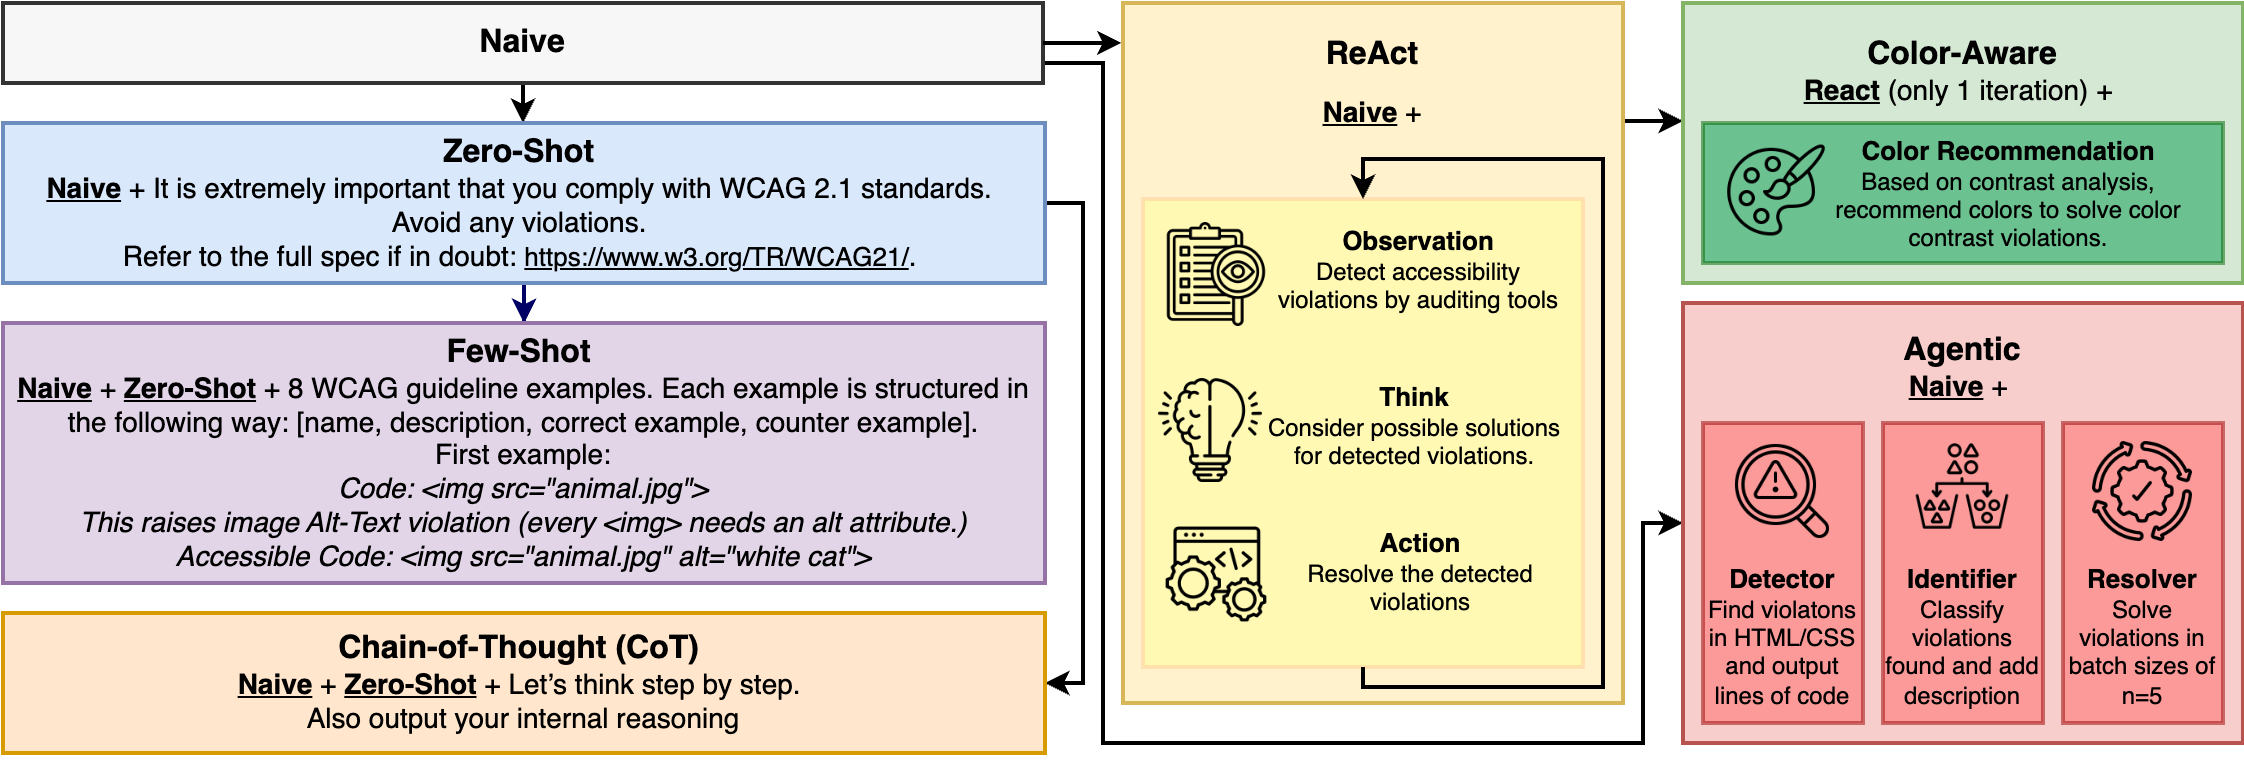
\includegraphics[width=0.85\linewidth]{figures/prompts_new_new.png}
  \caption{Overview of the advanced prompting strategies.}
  \label{fig:prompts_new} 
\end{figure}


\begin{itemize}
    \item Naive Prompting (Baseline): Without any explicit accessibility instructions, the model is
    instructed to generate HTML/CSS code from a webpage screenshot.
    \item Zero-Shot Prompting: The MLLMs are explicitly instructed to 
    generate accessible code by adding the instruction \textit{``comply with WCAG 2.1 standards''}, 
    as shown in Fig.~\ref{fig:prompts_new}. 
    This explores the model's ability to generalize accessibility guidelines 
    only based on an instruction and without examples.
    \item Few-Shot Prompting: This strategy resembles the zero-shot prompt,
    but is enriched with several examples of WCAG 2.1 guidelines, combined 
    with a description of the task, an incorrect code snippet and a 
    corresponding correct code snippet.
    The examples are sourced from the ARIA Authoring Practices Guide 
    (by W3C)~\cite{web:w3c_examples} and Accessible Components by Gov.uk 
    Design System~\cite{web:govuk}, which are known for their accessibility
    best practices.
    Eight examples, which differ in their content (e.g., image alt-text, 
    form labels, landmarks) are manually collected. They serve as an 
    additional context for the model to lead the models towards a more 
    accessible code generation.
    \item Chain-of-Thought Prompting: As shown in Fig.~\ref{fig:prompts_new}, 
    the prompt encourages the model to think step-by-step. 
    The objective is to guide the model to describe its 
    considerations in a structured plan and finally output the code.
    This helps to show intermediate reasoning steps that possibly 
    highlight accessibility-aware thinking.
    \item ReAct Prompting: 
    This strategy first instructs the model to generate HTML/CSS code, 
    according to the naive prompt and then critique its accessibility
    violations detected by the automated tools. As shown in 
    Fig.~\ref{fig:prompts_new}, the model is then asked to revise
    all violations found, prioritize those with the highest 
    severity and output the revised code.
    This multi-step approach evaluates the capability of the model to 
    self-correct and iteratively apply accessibility standards. 
    Each self-refinement loop runs for three iterations or until 
    no further violations are detected.
    \item Color Aware Prompting: 
    As previous RQs have shown, color contrast violations are a common 
    issue in MLLM-generated code. Due to their mathematical nature, they
    can be difficult to solve. Therefore, this strategy extends the ReAct 
    prompting by adding a color-aware step. It uses a pre-processing 
    step which extracts the color values from the screenshot, analyzes 
    the color contrast violations found and provides the model with a 
    possible solution for each violation. Similar to the ReAct prompting,
    the model is then instructed to output the revised code. 
    By basing the model on extracted color values and recommended 
    replacements that satisfy WCAG thresholds, the objective is to 
    decrease color-contrast accessibility violations. The model is 
    directed to generate code that maintains visual consistency while 
    utilizing compliant color pairs by supplying this analysis and 
    asking for a revision.
    Note that the refinement loop runs only for one iteration.
    \item Agentic Prompting: 
    As prior research~\cite{wu2023autogen} has shown, the use of multi-agent 
    systems, where each agent has a specific task, can lead to better
    results in complex tasks. Therefore, this strategy splits the 
    task of creating accessible code into three agents: The 
    \textit{Detector} agent is designed to detect accessibility violations 
    in a generated code, instructed with the naive prompt. It outputs a list
    of snippets with violations, including their location in the code. The 
    second agent, the \textit{Identifier}, is responsible for classifying 
    the violations into their respective WCAG guidelines (e.g., 
    color contrast, landmarks, etc.) and enrich the each violation with 
    its severity level. The third agent, the \textit{Resolver}, is 
    instructed to resolve the list of violations in the code. In order to 
    prevent cascading errors, this agent is instructed to solve batches 
    of violations, having a size of \(n = 5\). The goal of this strategy 
    is to evaluate whether decomposing the task into smaller and more 
    manageable subtasks can improve the overall accessibility.
\end{itemize}

Note that all prompting techniques are tested on GPT and Gemini by using the 
same benchmark dataset.


\subsection{Results}
Table~\ref{tab:access-viol-models} presents

\begingroup
    \begin{table}[htbp]
  \centering
  \footnotesize
  \setlength{\tabcolsep}{2pt}
  \begin{tabular}{l *{2}{ccccc}}
    \toprule
    \multirow{2}{*}{\textbf{Technique}} &
      \multicolumn{5}{c}{\textbf{GPT}} &
      \multicolumn{5}{c}{\textbf{Gemini}} \\
    \cmidrule(lr){2-6}\cmidrule(l){7-11}
      & Average Violations & Total Violations & CodeSim & IR & IWIR
      & Average Violations & Total Violations & CodeSim & IR & IWIR \\
    \midrule
    Naive               & 13.75 & 729 & \underline{\textbf{88.96\%}} & 12.22\% & 47.10\%
                        & 15.45 & 819 & \underline{\textbf{87.12\%}} & 11.42\% & 47.70\% \\
    Zero-Shot           & 12.33 & 653 & 87.79\% & \textemdash & \textemdash
                        & 14.25 & 755 & 86.85\% & \textemdash & \textemdash \\
    Few-Shot            &  9.49 & 503 & 87.29\% & \textemdash & \textemdash
                        & 15.74 & 834 & 86.95\% & \textemdash & \textemdash \\
    Chain-of-Thought    & 10.04 & 532 & 87.91\% & \textemdash & \textemdash
                        & 14.28 & 757 & 86.80\% & \textemdash & \textemdash \\
    ReAct               & \underline{\textbf{0.68}} & \underline{\textbf{36}} & 86.94\% & \textemdash & \textemdash
                        & \underline{\textbf{2.77}} & \underline{\textbf{147}} & 86.16\% & \textemdash & \textemdash \\
    Color-Aware         & \textemdash & \textemdash & \textemdash & \textemdash & \textemdash
                        & \textemdash & \textemdash & \textemdash & \textemdash & \textemdash \\
    Agentic             & \textemdash & \textemdash & \textemdash & \textemdash & \textemdash
                        & \textemdash & \textemdash & \textemdash & \textemdash & \textemdash \\
    \bottomrule
  \end{tabular}
  \caption{Performance for advanced prompting techniques (including IR and IWIR).}
  \label{tab:access-viol-models}
\end{table}

\endgroup